\chapter{Sums of Combinatorial Games}
Assume we have two combinatorial games $\mathcal{G}_1$ and $\mathcal{G}_2$.
One may form another game played as follows: the initial position of the new game
consists of the pair of initial positions of $\mathcal{G}_1$ and $\mathcal{G}_2$,
players alternate moves, and on each turn a player make a move in one of the game
leaving the position in the second untouched.  The new game is called
\emph{sum of $\mathcal{G}_1$ and $\mathcal{G}_2$}.

Let us give a formal definition.
\begin{definition}
    Let $G_1 = (V_1, F_1)$ and $G_2 = (V_1, F_2)$ be directed graphs.
    We say that $G$ is the sum of $G_1$ and $G_2$, denoted $G_1 + G_2$, is
    a graph $(V_1 \times V_2, F)$  such that
    \[
        F(x_1, x_2) =
            \set[y_1 \in F_1(x_1)]{(y_1, x_2)} \cup
            \set[y_2 \in F_2(x_2)]{(x_1, y_2)}.
    \]
\end{definition}
\Cref{figure:sum-of-graphs-G1-G2} gives an example of this operation.

\begin{figure}
    \centering
    \subfloat[$G_1$\label{figure:sum-of-graphs-G1}]{
        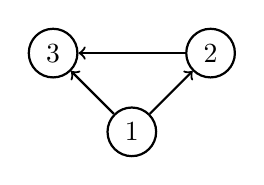
\begin{tikzpicture}[thick]
          \node[circle, draw, minimum size=6pt] (v1) at (0,0) {$1$};
          \node[circle, draw, minimum size=6pt] (v2) at (1,1) {$2$};
          \node[circle, draw, minimum size=6pt] (v3) at (-1,1) {$3$};


          \draw[->] (v1) -- (v2);
          \draw[->] (v1) -- (v3);
          \draw[->] (v2) -- (v3);
        \end{tikzpicture}
    }
    \qquad\qquad
    \subfloat[$G_2$\label{figure:sum-of-graphs-G2}] {
        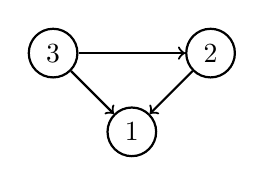
\begin{tikzpicture}[thick]
          \node[circle, draw, minimum size=6pt] (v1) at (0,0) {$1$};
          \node[circle, draw, minimum size=6pt] (v2) at (1,1) {$2$};
          \node[circle, draw, minimum size=6pt] (v3) at (-1,1) {$3$};


          \draw[->] (v2) -- (v1);
          \draw[->] (v3) -- (v1);
          \draw[->] (v3) -- (v2);
        \end{tikzpicture}
    }
    \qquad\qquad
    \subfloat[$G_1 + G_2$\label{figure:sum-of-graphs-G1-G2}] {
        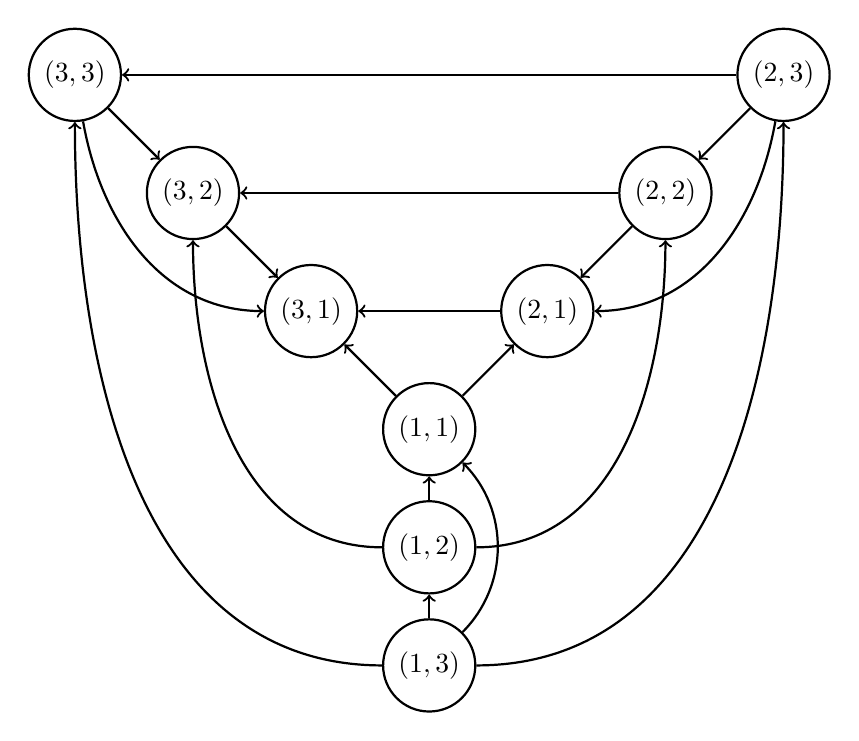
\begin{tikzpicture}[thick]
          \node[circle, draw, minimum size=6pt] (v11) at (0, 0)  {$(1, 1)$};
          \node[circle, draw, minimum size=6pt] (v21) at (1.5, 1.5)  {$(2, 1)$};
          \node[circle, draw, minimum size=6pt] (v31) at (-1.5, 1.5) {$(3, 1)$};
          \node[circle, draw, minimum size=6pt] (v12) at (0, -1.5) {$(1, 2)$};
          \node[circle, draw, minimum size=6pt] (v22) at (3, 3)  {$(2, 2)$};
          \node[circle, draw, minimum size=6pt] (v32) at (-3, 3) {$(3, 2)$};
          \node[circle, draw, minimum size=6pt] (v13) at (0,-3)  {$(1, 3)$};
          \node[circle, draw, minimum size=6pt] (v23) at (4.5,4.5)  {$(2, 3)$};
          \node[circle, draw, minimum size=6pt] (v33) at (-4.5,4.5) {$(3, 3)$};


          \draw[->] (v11) -- (v21);
          \draw[->] (v11) -- (v31);
          \draw[->] (v21) -- (v31);
          \draw[->] (v12) to[out = 0, in = -90] (v22);
          \draw[->] (v12) to[out = 180, in = -90] (v32);
          \draw[->] (v22) -- (v32);
          \draw[->] (v13) to[out = 0, in = -90] (v23);
          \draw[->] (v13) to[out = 180, in = -90] (v33);
          \draw[->] (v23) -- (v33);
          \draw[->] (v12) -- (v11);
          \draw[->] (v13) to[out = 45, in = -45] (v11);
          \draw[->] (v13) -- (v12);
          \draw[->] (v22) -- (v21);
          \draw[->] (v23) to[out = -100, in = 0] (v21);
          \draw[->] (v23) -- (v22);
          \draw[->] (v32) -- (v31);
          \draw[->] (v33) to[out = -80, in = 180] (v31);
          \draw[->] (v33) -- (v32);
        \end{tikzpicture}
    }
    \caption{\Cref{figure:sum-of-graphs-G1-G2} depicts sum of graphs
        from \Cref{figure:sum-of-graphs-G1} and \Cref{figure:sum-of-graphs-G2}.
    }
\end{figure}


Another example is given by the game of Nim; it is easy to see that
$2$-pile Nim is a sum of two $1$-pile Nims. This observation allows to generalize
Bouton's Theorem (\Cref{theorem:bouton}).
\begin{theorem}[Sprague--Grundy Theorem]
    Let $G_1$ and $G_2$ be some graphs and $g_1$ and $g_2$ be corresponding
    Sprague--Grundy functions. Then the graph $G_1$ and $G_2$ has a
    Sprague--Grundy function $g$ such that
    $g(x_1, x_2) = g_1(x_1) \bitwisexor g_2(x_2)$.
\end{theorem}
\begin{proof}
    Let $G_1 = (V_1, F_1)$, $G_2 = (V_2, F_2)$, and $G = G_1 + G_2$.
    Consider some $x_1 \in V_1$ and $x_2 \in V_2$.
    Let $a = g_1(x_1) \bitwisexor g_2(x_2)$. To prove the statement we need to
    show that
    \begin{enumerate}
        \item for any $0 \le b < a$, there is $(y_1, y_2) \in F(x_1, x_2)$ such
            that $g(y_1, y_2) = b$;
        \item for any $(y_1, y_2) \in F(x_1, x_2)$, $g(y_1, y_2) \neq a$.
    \end{enumerate}

    We start from proving the first statement.
    Let us fix some $0 \le b < a$ and let $c = a \bitwisexor b$.
    Let $g_i(x_i) = (p_{i, \ell}, \dots, p_{i, 0})$ for each $i \set{1, 2}$ and
    $c = (1, q_{k - 1}, \dots, q_0)$ where $k \le \ell$.
    For some $j \in \set{1, 2}$, $p_{j, k} = 1$ since
    $a = g_1(x_1) \bitwisexor g_2(x_2)$. Without loss of generality $j = 1$.
    Hence, $c \bitwisexor g_1(x_1) < g_1(x_1)$, whence there is $x'_1$ such
    that $g_1(x'_1) = c \bitwisexor g_1(x_1)$. As a result, there is a move in
    $G$ from $(x_1, x_2)$ to $(x'_1, x_2)$ and
    $g(x'_1, x_2) = g_1(x'_1) \bitwisexor g_2(x_2) =
        c \bitwisexor g_1(x_1) \bitwisexor g_2(x_2) =
        c \bitwisexor a = b$.

    To prove the second statement, assume that there is
    $(y_1, y_2) \in F(x_1, x_2)$ so that $g(y_1, y_2) = a$. Without loss of
    generality we may assume that $x_2 = y_2$. Hence,
    $0 = g(y_1, x_2) \bitwisexor g(x_1, x_2) = g_1(y_1) \bitwisexor g_1(x_1)$.
    However, $g_1(y_1) \neq g_1(x_1)$ since there is a move from $x_1$ to $y_1$.
    Therefore $g_1(y_1) \bitwisexor g_1(x_1) \neq 0$ which is a contradiction.
\end{proof}

The simple example of an application of this theorem is the analisis of the
following game.
\begin{game}
\label{game:subtraction-1-2-3-out-of-10-11}
  Alice and Bob have two piles with $10$ and $11$ chips respectively.
  They take turns and remove $1$, $2$, or $3$ chips from one of the piles.
  If one of them cannot make a move he/she loses.
\end{game}
We need to determin who wins if both of them are playing optimally?

To give an answer for this question we start with a simpler game,
a subtraction game with a subtraction set $\set{1, 2, 3}$. It is easy to see
that $g : \N_0 \to \set{0, 1, 2}$ such that
\[
  g(x) =
  \begin{cases}
      0 & x \equiv 0 \pmod{3} \\
      1 & x \equiv 1 \pmod{3} \\
      2 & x \equiv 2 \pmod{3}
  \end{cases}
\]
is a Sprague--Grundy function for a subtraction game with a subtraction set
$\set{1, 2, 3}$.
It is also clear that \Cref{game:subtraction-1-2-3-out-of-10-11} is a sum of
two subtraction games with a subtraction set $\set{1, 2, 3}$.
